% Bsp. eines Hauptteils

\chapter{Ziel des Projekts}
\label{sec:grundl}
Ziel des Projekts ist es, eine Software zu entwickeln, die den IO von Anwendungen analysiert. Die Software soll sich dabei zwischen das zu analysierende Programm und das Betriebssystem schalten und s\"amtlichen IO abfangen. Der IO des Programms soll anschliessend gespeichert und graphisch aufbereitet werden. Die Software soll dabei interaktiv sein. Das bedeutet, es soll mit der Software m\"oglich sein, gezielt nach IO-Engp\"assen in einer Anwendung zu suchen.\newline\newline
Im ersten Schritt sollen dabei bestehende Softwarel\"osungen evaluiert werden. Im zweiten Schritt geht es dann darum, eine eigene Software zu entwickeln, welche die oben genannten Forderungen erf\"ullt. Anforderungen an die Software sind sowohl eine portable Entwicklung, als auch Thread-Sicherheit.

\chapter{Stand der Technik}
\label{sec:tech}
Im Rahmen der Forschungsarbeit erfolgte zun\"achst eine Marktrecherche, welche Softwarel\"osungen zum Tracing von IO bereits auf dem Markt sind. Dar\"uber hinaus wurden diese L\"osungen bez\"uglich ihrer Funktionalit\"at evaluiert. Wichtigstes Kriterium bei der Marktrecherche ist, dass es sowohl m\"oglich ist POSIX-IO zu untersuchen, als auch MPI-IO. Dar\"uber hinaus soll die Analyse zur Laufzeit ohne Recompilieren des Codes m\"oglich sein.
\section{Darshan}
Darshan ist ein Programm zur Analyse von POSIX-IO und MPI-IO. Mit Darshan kann ein PDF-Report des IO von Programmen erstellt werden. Bei dynamisch gelinkten Programmen ist dies zur Laufzeit m\"oglich, bei statisch gelinkten Programmen ausschliesslich beim Bau des Programms.\newline
Darshan besteht aus zwei Programmen. Mit Darshan-Runtime werden die Informationen \"uber den IO eines Programms gesammelt und gespeichert, mit Darshan-Util werden diese aufbereitet und dargestellt.
\subsection{Funktionsweise}
Das Sammeln von Informationen zur Laufzeit von Programmen geschieht \"uber die Systemvariable LD\_PRELOAD. Mit dieser ist es m\"oglich Features in ein Prorgamm einzuschleusen. Beim Laden von Shared Libraries wird dabei zun\"achst nicht die eigentliche Bibliothek geladen, sondern diese, welche unter LD\_PRELOAD angegeben wurde. Damit wird dann die Darshan-Bibliothek geladen, welche die IO-Befehle speichert und diese anschliessend an die eigentlichen Bibliotheken weitergibt. Die Funktionsweise von Darshan f\"ur dynamisch gelinkte Programme ist in Abbildung \ref{fig:darshan} dargestellt. Die Bibliothek libdarshan.so wird dabei vom zu untersuchenden Programm \"uber LD\_PRELOAD geladen. Diese speichert alle MPI-IO- und POSIX-IO-Befehle in Log-Dateien. Diese Log-Dateien k\"onnen anschliessend mit Darshan-Util ausgewertet werden. Dabei wird ein PDF-Report kreiert in welchem in Diagrammen u.a. dargestellt wird, wieviele IO-Operationen jeweils durchgef\"uhrt wurden und welche Datenmengen dabei verarbeitet wurden.

\begin{figure}[h]
	\centering
	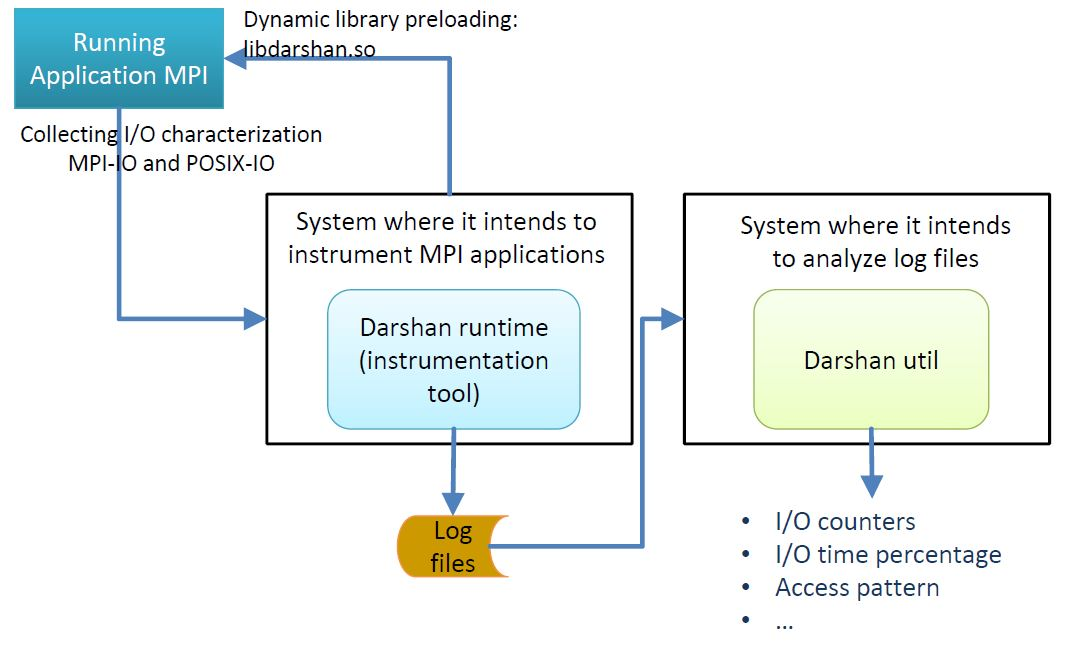
\includegraphics[width=12cm]{fig/Darshan.jpg}
	\caption{Darshan Aufbau \cite{Mendez.23.06.2016}}
	\label{fig:darshan}
\end{figure}

Das Analysieren von statisch gelinkten Programmen funktioniert \"ahnlich wie bei VampirTrace mit Compiler-Wrappern. Diese werden beim Bau anstatt der eigentlichen Compiler aufgerufen. Die Wrapper werten das Programm dann aus und schreiben die Log-Dateien. Anschliessend werden die eigentlichen Compiler aufgerufen. \cite{ArgonneNationalLaboratory.22.01.2019}\cite{ArgonneNationalLaboratory.19.01.2019}
\subsection{Fazit}
Darshan ist ein hervorragendes Programm zur Analyse des IO von dynamisch gelinkten Programmen. Der Nachteil liegt dabei jedoch darin, dass der graphische Output nicht interaktiv ist. Es wird zwar ein PDF-Report kreiert, es ist jedoch nicht m\"oglich interaktiv gezielt nach Schwachstellen im Programm zu suchen. Dar\"uber hinaus k\"onnen statisch gelinkte Programme mit Darshan nicht zur Laufzeit ohne erneuten Bau untersucht werden, was ebenfalls einen gravierenden Nachteil darstellt. 
\section{VampirTrace}
VampirTrace ist ein Programm, welches von der Universit\"at Dresden zur urspr\"unglich Analyse von MPI-Programmen entwickelt wurde. Mittlerweile ist es ein Tool-Set zur Analyse von parallelen Programmen im HPC-Bereich. Mit VampirTrace kann sowohl MPI-IO als auch POSIX-IO untersucht werden. F\"ur die Analyse von Programmen ist es notwendig, diese mithilfe von VampirTrace-Compiler-Wrappern neu zu bauen. Im Makefile m\"ussen dabei die Compiler durch die Compiler-Wrapper von VampirTrace ersetzt werden. Diese rufen dann wiederum die eigentlichen Compiler auf. Die gebauten Programme k\"onnen anschliessend zur Laufzeit mit VampirTrace analysiert werden. Eine Untersuchung zur Laufzeit ohne neuen Bau ist nicht ohne weiteres m\"oglich.\newline\newline
Die gewonnenen Daten werden von VampirTrace in einer Log-Datei im Open-Trace-Format (OTF) gespeichert. Diese Log-Dateien k\"onnen anschliessend mit Tools, die den Umgang mit OTF beherrschen, visualisiert werden. Am besten eignet sich hierzu das Tool Vampir, welches ebenfalls von der Universit\"at Dresden zu diesem Zweck entwickelt wurde.
\cite{TUDresden.2016}
\section{Ludalo}
Mit Ludalo ist es m\"oglich Lustre-Metadaten-Operationen zu analysieren.
\cite{Berger.30.07.2014}
\section{TAU}
Tau ist eine Software, entwickelt von der University of Oregeon, zur Analyse von parallelen Applikationen. Eine IO-Analyse ist dabei sowohl f\"ur POSIX-IO, als auch f\"ur MPI-IO m\"oglich. Die von TAU generierten Daten k\"onnen im OTF-Format gespeichert und anschliessend mit Vampir visualisiert werden. Die Analyse erfolgt entweder durch das Recompilieren des Codes oder durch das Laden einer Bibliothek mit LD\_PRELOAD. Hinsichtlich der Funktionalit\"at wurde TAU in diesem Projekt nicht weiter evaluiert.
\cite{Shende.03.05.2017}\cite{Shende.2011}

\section{Fazit}
Keines der untersuchten Programme enth\"alt alle Features, welche in diesem Projekt gew\"unscht sind. Darshan trifft die Anforderungen jedoch am ehesten. Damit kann sowohl MPI-IO als auch POSIX-IO analysiert werden. Allerdings ist dabei keine interaktive Bedienung m\"oglich. Dasselbe ist bei VampirTrace auch der Fall. Damit kann zwar ebenfalls MPI-IO und POSIX-IO analysiert werden, jedoch ist auch hierbei keine interaktive Bedienung vorhanden. Aus diesem Grund soll in diesem Projekt eine Software entwickelt werden, welche die Features von Darshan und VampirTrace mit einer interaktiven Bedienung vereint.

\chapter{Entwicklung einer eigenen Software}
\section{Architektur}
\label{sec:real}

\section{Umsetzung}
\label{sec:umsetz}

\chapter{Aktueller Stand}
\label{sec:ergeb}

